\documentclass[12pt]{article}
\usepackage[utf8]{inputenc}
\usepackage{amsmath}
\usepackage[spanish]{babel}
\usepackage[margin=25mm]{geometry}
    %\hyphenation{thatshouldnot}
\usepackage{graphicx}
    \graphicspath{{images/}}
\usepackage{tikz}
    \usetikzlibrary{shapes,arrows,positioning}
\usepackage{float}
\usepackage{listings} 
\renewcommand{\lstlistingname}{Código}
\usepackage{parskip}
\usepackage{hyperref}

\definecolor{codegreen}{rgb}{0,0.6,0}
\definecolor{codegray}{rgb}{0.5,0.5,0.5}
\definecolor{codepurple}{rgb}{0.58,0,0.82}
\definecolor{backcolour}{rgb}{0.95,0.95,0.92}

\lstdefinestyle{mystyle}{
    backgroundcolor=\color{backcolour}, commentstyle=\color{codegreen},
    keywordstyle=\color{magenta},
    numberstyle=\tiny\color{codegray},
    stringstyle=\color{codepurple},
    basicstyle=\ttfamily\footnotesize,
    breakatwhitespace=false,
    breaklines=true,
    captionpos=b,
    keepspaces=true,
    numbers=left,
    numbersep=5pt,                  
    showspaces=false,                
    showstringspaces=false,
    showtabs=false,                  
    tabsize=2,
    frame = single, 
}
\lstset{style=mystyle}

\begin{document}

\begin{titlepage}
    \centering
    {\scshape\LARGE Universidad Católica de Santa María \par}
    \vspace{3em}
    
\includegraphics[width=0.25\textwidth]{images/ucsm.png}\par\vspace{3em}
    \vspace{1cm}
    {\scshape\Large Escuela Profesional de Ingeniería Electrónica \par}
    \vspace{1.5cm}
    {\huge\bfseries Informe 4NEC2\par}   % título del proyecto
    \vspace{2cm}
    \large
    {\bfseries Curso:} Software de Telecomunicaciones\par
    {\bfseries Alumno:} Luis Orlando Figueroa Morales\par
    {\bfseries Docente:} Ing. Mario Urrutia Espinoza 

    \vfill

    {\small Arequipa - 2021\par}
\end{titlepage}

\tableofcontents

\newpage

\section{Introducción}

4NEC2 es un programa libre para modelizar antenas. Además de ser una
herramienta potente para crear, ver optimizar y probar estructura de antenas en
2D y 3D que también genera, muestra y compara campos cercanos y lejanos de
radiación. El código fuente esta escrito en el lenguaje de programación Fortran.

4NEC2 por sus siglas en inglés: ``The Numerical Electromagnetics Code (NEC-2)''
es un programa orientado al usuario para el análisis de respuesta
electromagnéticas de antenas y de otras estructuras metálicas. Esta hecho a
través de distintos métodos numéricos de solución con ecuaciones integrales
para para las corrientes inducidas en la estructura por fuentes o campos
incidentes.

El código fuente en el cual esta hecho 4NEC2 combina varias ecuaciones
integrales para superficies suaves con una especializada en cables para proveer
precisión para el modelamiento en estructuras de un ancho rango. Los modelos
deben incluir redes no radiantes y líneas de transmisión conectadas a partes de
la estructura, con conductores perfectos e imperfectos.

Algunas de las herramientas que vienen en 4NEC2 son el Optimizer y Sweeper con
el cual se pueden hacer optimizaciones en la antena cuando se ejecutan barridos
dé frecuencia haciendo que se generen gráficos de líneas de impedancia, ROE,
ganancia, relación F/B de estilo lineal y logarítmico. Haciendo el Sweeper (o
barrido) se puede mostrar de manera gráfica.

\begin{figure}[H]
\centering
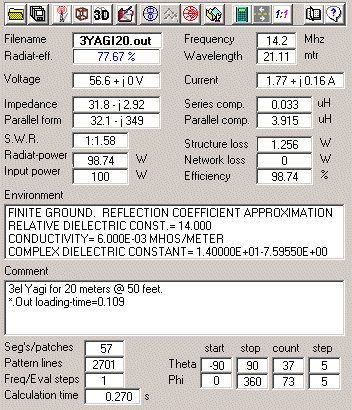
\includegraphics[width=.4\linewidth]{images/image002.png}
\caption{Ventana principal de 4NEC2.}
\end{figure}

\section{Características}

Algunas de las características que este software nos detalla en su
documentación (https://www\-.qsl.net/4nec2/) son:

\begin{itemize}
\item Las gráficas en 2D y 3D de visualización de estructuras geométricas.
\item Opción para arrastrar y soltar para poder modelar antenas.
\item Visualización interactiva de la Carta de Smith para barridos de
frecuencia.
\item Archivo de ayuda de manera contextual.
\end{itemize}

\section{Modelamiento de la antena}

Para el modelamiento de antenas debemos considerar distintos parámetros a tomar
en cuenta para diseñar una antena. Como se sabe hay fórmula sencillas que se
utilizan para hallar diseño de antenas (por ejemplo las dipolo) pero colocarlas
en un software como NEC2 facilita estos cálculos pues solo se pondrían ciertos
parámetros (como frecuencia y rango de radiación) para que el mismo software
nos haga el análisis a partir del conocimiento previo que tenemos del programa.

NEC2 usa un análisis básico de la antena basado en el ``método de momentos'',
una técnica matemática donde subdivida una antena en pequeños segmentos para
calcular las propiedades mas apropiadas para cada caso. Los resultados pueden
ser sencillamente ajustados a las ecuaciones de ingeniería para resistencia del
material, carga del elemento y efectos de la tierra. 

\subsection{Modelamiento con Geometry Edit}

Con Geometry Editor se puede establecer la estructura geométrico de la antena.
Esta herramienta se encuentra dentro de al ventana Main en settings y se marca
Geometry Edit. Después de esto se presiona edit NEC and input file donde carga
un ejemplo.

Por ejemplo, si se quiere modelar un dipolo de $\lambda$.

\begin{figure}[H]
\centering
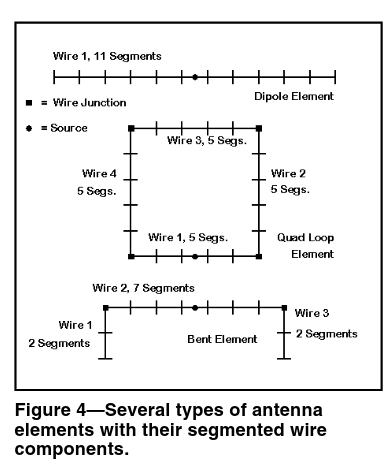
\includegraphics[width=.4\linewidth]{images/Captura de pantalla de 2021-09-12 23-21-26.png}
\end{figure}

En esta figura se pueden ver los distintos elementos, un dipolo, antenas
cúbicas de bucle y elementos doblados. Para formas que no son rectas en 4NEC2 se
debe poner un aproximado ya que es una figura no recta.

\section{Interfaz de usuario para 4nec2}

Al inicio el usuario tiene cuatro ventanas principales (y también accesos
rápidos a dichas ventanas. Las cuales son:

\begin{enumerate}
    \item Main (F2).
    \item Geometry (F3).
    \item Pattern (F4).
    \item Impedance (Imp/SWR/Gain) (F5).
\end{enumerate}

A continuación se puede ver una captura de pantalla de una maquina virtual con
4NEC2 instalado, donde se pueden apreciar las 4 ventanas ya abiertas.

\begin{figure}[H]
    \centering
    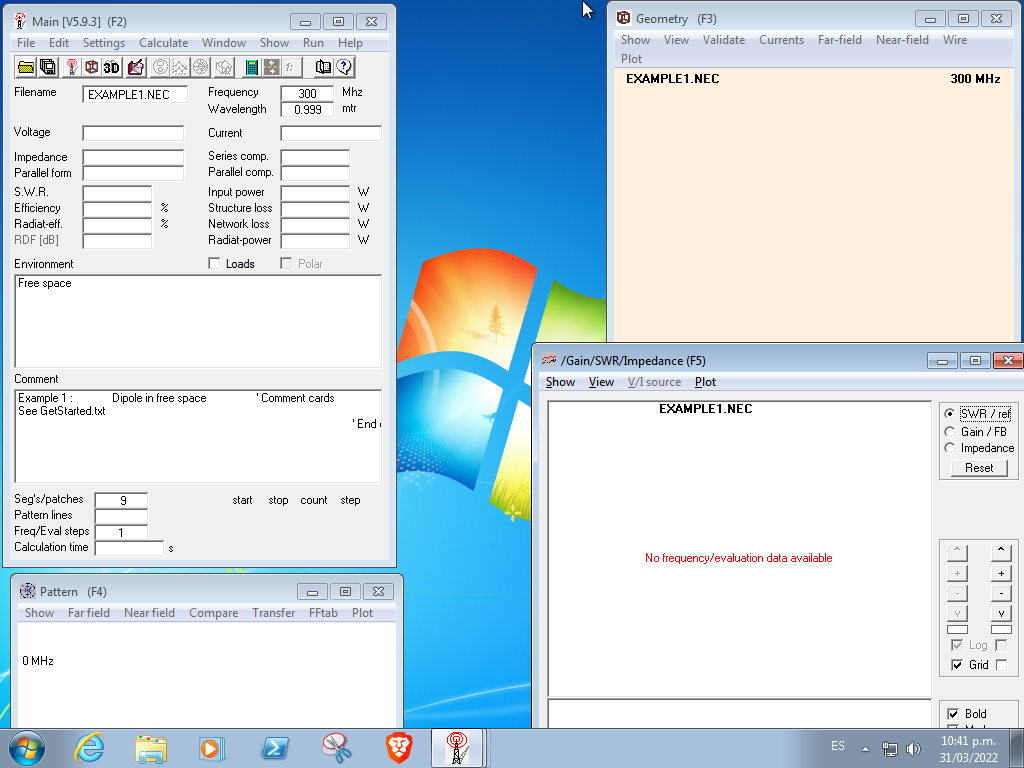
\includegraphics[width=.8\linewidth]{images/Screenshot_win7_2022-03-31_22_41_34.png}
    \caption{Captura de pantalla de las 4 ventanas ya ejecutadas.}
\end{figure}

\section{Como modelar antenas}

Lo importante antes de comenzar haciendo la modelación de las antenas es
conocer cual es nuestro entorno como por ejemplo saber que tipos de archivos
vamos a usar a editar, como lo veremos a continuación.

Hay muchas guías en internet pero en esta ocasión usaremos una guía disponible
en la página \href{https://leanpub.com/4nec2definitiveguide/read}{leanpub}.

\subsection{Archivos NEC}
Lo primero para poder hacer el modelamiento de la antena es reconocer como es
un archivo NEC (Numerical Electromagnetics Code ó Código Numérico
Electromagnético).

\begin{lstlisting}[language=,caption=Ejemplo de un archivo .NEC de una antena
logarítmica periódica.]
CM TESTEX5
CM 12 ELEMENT LOG PERIODIC ANTENNA IN FREE SPACE
CM 78 SEGMENTS. SIGMA=O/L RECEIVING AND TRANS. PATTERNS.
CM DIPOLE LENGTH TO DIAMETER RATIO=150.
CE TAU=0.93. SIGMA=0.70. BOOM IMPEDANCE=50. OHMS.
GW 1 5 0.0000 -1.0000 0.0000000 0.00000 1.0000 0.000 .00667
GW 2 5 -.7527 -1.0753 0. -.7527 1.0753 0. .00717
GW 3 5 -1.562 -1.1562 0. -1.562 1.1562 0. .00771
GW 4 5 -2.4323 -1.2432 0. -2.4323 1.2432 0. .00829
GW 5 5 -3.368 -1.3368 0. -3.368 1.3368 0. .00891
GW 6 7 -4.3742 -1.4374 0. -4.3742 1.4374 0. .00958
GW 7 7 -5.4562 -1.5456 0. -5.4562 1.5456 0. .0103
GW 8 7 -6.6195 -1.6619 0. -6.6195 1.6619 0. .01108
GW 9 7 -7.8705 -1.787 0. -7.8705 1.787 0. .01191
GW 10 7 -9.2156 -1.9215 0. -9.2156 1.9215 0. .01281
GW 11 9 -10.6619 -2.0662 0. -10.6619 2.0662 0. .01377
GW 12 9 -12.2171 -2.2217 0. -12.2171 2.2217 0. .01481
GE
FR 0 0 0 0 46.29 0.
TL 1 3 2 3 -50.
TL 2 3 3 3 -50.
TL 3 3 4 3 -50.
TL 4 3 5 3 -50.
TL 5 3 6 4 -50.
TL 6 4 7 4 -50.
TL 7 4 8 4 -50.
TL 8 4 9 4 -50.
TL 9 4 10 4 -50.
TL 10 4 11 5 -50.
TL 11 5 12 5 -50. ,0.,0.,0.,.02
EX 0 1 3 10 1 
RP 0 37 1 1110 90. 0. -5. 0.
EN
\end{lstlisting}

\section{Facilidades de procesado}

Se tiene dos formas para la simulación con NEC2, la primera es usando el editor
geométrico para desarrollar y modificar el modelado de una antena, es necesario
que se tenga por lo menos una variable a optimizar, estas variables pueden
estar en el bloc de notas o en el editor NEC2, el cual sería el modelado en
bloc de notas editor ``notepad''.

\section{Diseñando una antena}

Se pueden realizar dos tipos de diseño en el software, uno es mediante la
herramienta ``Geometry Edit'', en donde se puede establecer una estructura
geométrica y la otra es mediante la herramienta de ``Notepad ''.

\subsection{Modelado con Geometry Edit}

Con este tipo de modelado se establece la estructura geométrica de una antena.

Para poder modelar se debe entrar a la ventana ``Main'' en settings y despu\'es
presionar en ``Edit NEC and input file''.

Se debe poner las propiedades de la antena, para esto se har\'a un ejemplo de
modelado de un dipolo \(\lambda/2\). para esto mencionaremos dos importantes
par\'ametros:

\begin{itemize}%Can change for enumerate
    \item Settings - Length Unit - Meters (en la ventana Main).
    \item Options - Set Segmentation - medium (en la ventana Geometry Edit).
\end{itemize}

Pasos para el modelado de la antena:

\textbf{Especificando diseño de la antena}.

Colocar una frecuencia de 29.98 Mhz (\(\lambda=10m\)).

\textbf{Añadir hilos} 

Crear un nivel XZ haciendo click en el bot\'on XZ. Luego introducir el hilo
presionando el bot\'on del dibujo del hilo para habilitar se presiona el
bot\'on ADD, el cual deber\'ia activarse en verde y la casilla Y (-). Se
introduce un valor en Y el cual nos dar\'a la altura o profundidad.  Para este
ejemplo se tomar\'a una profundidad de 0 m. El grosor de la rejilla se ajusta
en la barra ``grid'' que aparece en la barra superior derecha. Para este
ejemplo se colocar\'a en 0.1m. Y para este ejemplo se colocar\'a un hilo desde
X=2.5m hasta X=-2.5m con un valor de Z=5m arrastrando el hilo del rat\'on con
el bot\'on izquierdo pulsado entre los puntos. Finalmente, el radio del hilo
debe ser seleccionado, de momento, a 1 mm. El tamaño de la ventana se puede
ajustar en la barra de zoom para tener un mejor manejo del programa.

\textbf{Agregar una fuente}

Con el bot\'on Add presionado, se pulsar\'a el bot\'on de la fuente a añadir.

Presionando en cualquier punto de la ventana de edici\'on har\'a que aparezca el
s\'imbolo de la fuente, la cual se podr\'a colocar en cualquier punto deseado.
En el caso del ejemplo que se est\'a aplicando lo centraremos en el hilo que se
encuentra en la posici\'on Y=0, Z?5, X=0. las fuentes solo pueden situarse
sobre los hilos. Para este ejemplo se tomar\'a una fuente de valor
\texttt{1.0+j0.0 V} y \texttt{1.0 V}.

\textbf{Conductividad de los hilos}

En esta simulaci\'on haremos nuestra antena con alambres de \textit{cobre} y
para ello se presionar\'a el bot\'on load (el s\'imbolo de RLC). Colocando la
carga en uno de los hilos, cerca de la fuente.

Despues se cambian las condiciones del hilo Par RLC a Wire-Ld y se selecciona
el cobre. Se ve como el segmento cobre \textit{copper} y se ve como se el
segmento apropiado del hilo de color anaranjado. Ahora, para cargar solo un
hilo se deber\'a colocar la opci\'on \textit{single wire}. 

\textbf{Desplazar/voltear/escalar antenas}

Para determinar el radio de la antena se debe marcar el bot\'on  select object
y el bot\'on wire geometry seleccionando un hilo, se tornar\'a de color rojo.
Posteriormente se introduce un hijo (puede ser de un radio \#7).

Usando este modo los hilos o las fuentes (y cargas) pueden ser desplazados o
girados, para realizar esto solo se debe seleccionar el hilo.

\textbf{Determinaci\'on de los par\'ametros de la tierra}

Por defecto se representa el espacio de la antena al aire libre, para ponerla
en segundo plano se debe marcar el bot\'on de Ground Params y elegir el tipo de
tierra que se desee entre  \textit{``Free Space, Fast Ground, Perf Ground, Real
Ground, Mininec Ground''}.

Para determinar los par\'ametros de la tierra se debe. Se elige los tipos de
tierra \textit{Clay/Forest}, el cual indica un promedio de arcilla y con
vegetaci\'on. Por defecto, la conductividad y la constante del diel\'ectrico
vienen fijadas a 0.005 S y 13 respectivamente.

<++> 

Para iniciar NEC2-Maschine se debe presionar el not\'on con s\'imbolo de
calculadora (o F7) despu\'es de guardar los datos. Aparecer\'a una ventana con
opciones para poder marcar. Si se quiere producir el diagrama de radiación para
campos lejanos se debe seleccionar ``Far Field pattern''. Seleccionamos la
casilla full para obtener el diagrama de radiación de aquella dirección en la
que nuestra antena radia mejor y tomamos una resolución de 5.

<++> 

En “Show NEC” podemos ver el desarrollo del programa en NEC. La explicación de
cada instrucción individual se desarrollará en capítulos posteriores. Si
marcamos el botón ``Comment/Wire data'' podemos escribir comentarios que
pudiéramos considerar luego al principio del código del programa. Los datos
concernientes al número de segmentos así como al número de hilos los
encontramos en segm-info.

\textbf{Consideraciones cuando se modela una antena}

\begin{itemize}%Can change for enumerate
    \item Los hilos deben conectarse por sus extremos. Si alguno se aproxima
	debe ser autom\'aticamente interconectado.
    \item Dos alambres no pueden cruzarse ni atravesar el \'area ya que pueden
	producir errores al conectarse.
    \item Cada hilo debe estar dividido en segmentos individuales. ``The
	NEC-maschine'' Consifdera cada segmento donde se desarrolla la potencia
	de una sinusoide, y supone que la uni\'on de ambos extremos de dos
	hijos de suman los flujos de ambos. Esto da un n\'umero finito de
	variables a determinar. La exactitud de este depende del n\'umero de
	segmentos, y al igual que el tiempo de computaci\'on.
\end{itemize}

\section{Verificaci\'on del modelo}

Tras simular este modelo, se debe comprobar los resultados, en un principio se
ven cuatro posibilidades. Se basa en la experiencia del usuario y en los datos
representados. Para un usuario que no posea conocimientos sobre alta frecuencia
le ser\'a muy difícil advertir si los resultados no son correctos. A
continuaci\'on se ver\'a cuatro posibilidades de comprobaci\'on de resultados
usando el ejemplo de modelo de $\lambda/2$.

Se debe examinar el patr\'on de radiaci\'on. Sabiendo que el dipolio radia en dos direcciones. Si este est\'a girando sobre la tierra no puede radiar hacia abajo. Usando estas afirmaciones se pueden observar en la figura <++>.

Posteriormente debemos mirar la eficiencia de la estructura de la antena. Por eficiencia entendemos la relación entre la potencia radiada y la proporcionada a la antena. Su valor se representa en la ventana Main. Ésta no puede ser mayor del
100\%. Si se diese este caso, la simulación sería incorrecta. Sin embargo, con una
estructura sin cargas es razonable contar con una eficiencia del 100\% puesto que no hay pérdidas. En el ejemplo del dipolo, que posee una carga, tenemos una eficiencia algo más pequeña del 100\%, en torno a 99,2\%. Esto parece realista y confirma la aceptación de los resultados. Si la eficiencia de la antena es muy pequeña, por debajo del 50\%, probablemente los resultados sean incorrectos.

\end{document}
